\documentclass{beamer}

\usepackage[textsize=footnotesize]{todonotes}
\usepackage{graphics} % resize table
\usepackage{tikz} % Precise image placement

\usetheme[compress]{Singapore}
\setbeamertemplate{footline}[frame number]
\setbeamercovered{transparent}
\beamertemplatenavigationsymbolsempty
%\setbeamertemplate{navigation symbols}{}



% These slides also contain speaker notes. You can print just the slides,
% just the notes, or both, depending on the setting below. Comment out the want
% you want.

%\setbeameroption{hide notes} % Only slides
%\setbeameroption{show only notes} % Only notes
%\setbeameroption{show notes on second screen=right} % Both

% To give a presentation with the Skim reader (http://skim-app.sourceforge.net) on OSX so
% that you see the notes on your laptop and the slides on the projector, do the following:
% 
% 1. Generate just the presentation (hide notes) and save to slides.pdf
% 2. Generate only the notes (show only nodes) and save to notes.pdf
% 3. With Skim open both slides.pdf and notes.pdf
% 4. Click on slides.pdf to bring it to front.
% 5. In Skim, under "View -> Presentation Option -> Synchronized Noted Document"
%    select notes.pdf.
% 6. Now as you move around in slides.pdf the notes.pdf file will follow you.
% 7. Arrange windows so that notes.pdf is in full screen mode on your laptop
%    and slides.pdf is in presentation mode on the projector.

% Give a slight yellow tint to the notes page
%\setbeamertemplate{note page}{\pagecolor{yellow!5}\insertnote}\usepackage{palatino}


\title{\uppercase{Electric Vehicle X Driving Range Prediction - EV X DRP}}
\subtitle{Relatório de progresso}
%\subtitle{}
\author{
	{\large David P. Coutinho \qquad Artur J. Ferreira} \\
	{\qquad \hspace{-1cm} david.coutinho@isel.pt \qquad arturj@isel.pt} \\
    {\vspace{1cm}}
    {\large David A. S. G. Albuquerque} \\
    {A43566@alunos.isel.pt}
}
\institute
{
	\vspace{0.5cm} \\
	{\normalsize Instituto Superior de Engenharia de Lisboa } \\
}
\date{
	\vspace{-0.75cm}
	3 de Maio de 2022
}

\usepackage[style=alphabetic]{biblatex}
\addbibresource{bibliography.bib}

\begin{document}

\begin{frame}[t,plain]
    \titlepage
\end{frame}

\begin{frame}
    \frametitle{Outline}
    \tableofcontents
\end{frame}

\section[Introdução]{Introdução}

\subsection[Diferenças entre veículos]{Diferenças entre veículos}
\begin{frame}
	\begin{itemize}
		\item Diferenças:
		\begin{itemize}
			\item Densidade de energia
			\item Quantidade de postos para atestar
		\end{itemize}
		\item Semelhanças:
		\begin{itemize}
			\item Estimação de autonomia
			\item Estimação do range de condução
		\end{itemize}
	\end{itemize}
	\frametitle{Introdução - Diferenças entre veículos}
	\begin{figure}[H]
		\begin{center}
			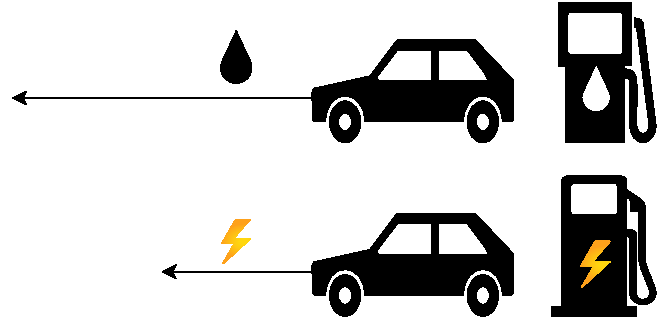
\includegraphics[scale=0.6]{./figures/ev_vs_gas_eRange.pdf}
		\end{center}
	\end{figure}
\end{frame}

%\note[itemize]{
%\item point 1
%\item point 2
%}

\subsection[\textit{eRange}]{\textit{eRange}}
\begin{frame}
\frametitle{Introdução - \textit{eRange}}

\begin{itemize}
	\item Cálculo das estimativas de distância de condução restante 
	que um veículo elétrico pode efetuar relativamente ao estado de 
	carga da sua bateria - \textit{eRange}
	\item Aliviar a ansiedade do condutor
\end{itemize}

\begin{figure}[H]
    \begin{center}
        \includegraphics[scale=0.20]{./figures/erange\_gauge}
		{\\EV dashboard \footfullcite{evDashboard}}
    \end{center}
\end{figure}
\end{frame}


\subsection[Que fatores influenciam o \textit{eRange}?]{Que fatores influenciam o \textit{eRange}?}
\begin{frame}
\frametitle{Introdução - Que fatores influenciam o \textit{eRange}?}

\begin{itemize}
	\item SOC (\textit{State of charge}) - indica o estado de carga da bateria
	\item Travagem regenerativa
	\item Consumo instantâneo
	\item Estado do ar condicionado / Aquecimento
	\item Condições atmosféricas
	\item Inclinação da estrada
	\item Tração dos pneus
	\item Carga a transportar
	\item (entre outros) 
\end{itemize}

\begin{tikzpicture}[remember picture, overlay]
	\node[left] at (current page.-10) 
	{
		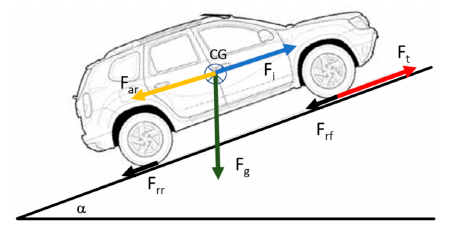
\includegraphics[width=0.65\textwidth]{./figures/forces.png}
		{\footfullcite{predictionOfeRangeCleared}}
	};
\end{tikzpicture}

\end{frame}

\subsection[Aplicação a desenvolver]{Aplicação a desenvolver}
\begin{frame}
\frametitle{Introdução - Aplicação a desenvolver}
\vspace{0.5cm}
\begin{figure}[H]
	{Fase de Geração}
	\begin{center}
		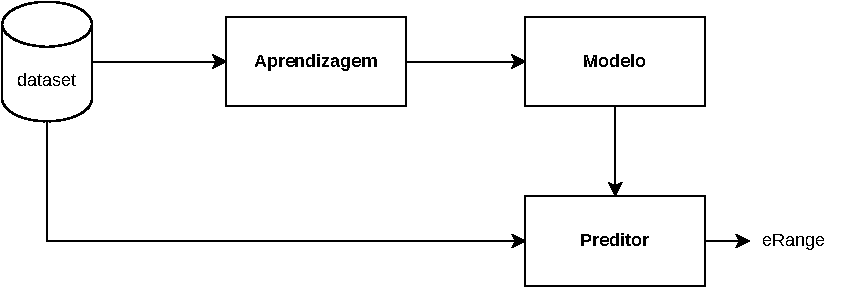
\includegraphics[scale=0.6]{./figures/objetivo_fase_de_geracao.pdf}
	\end{center}
\end{figure}

\begin{figure}[H]
	{Fase de Generalização}
	\begin{center}
		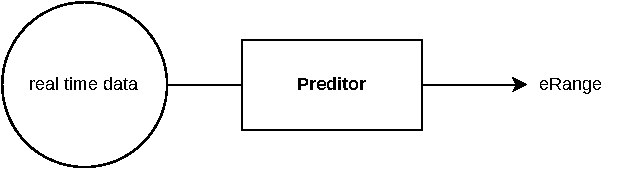
\includegraphics[scale=0.6]{./figures/objetivo_fase_de_generalizacao.pdf}
	\end{center}
\end{figure}

% \begin{tikzpicture}[remember picture, overlay]
% 	\node[below=3cm] at (current page.north) 
% 	{
% 		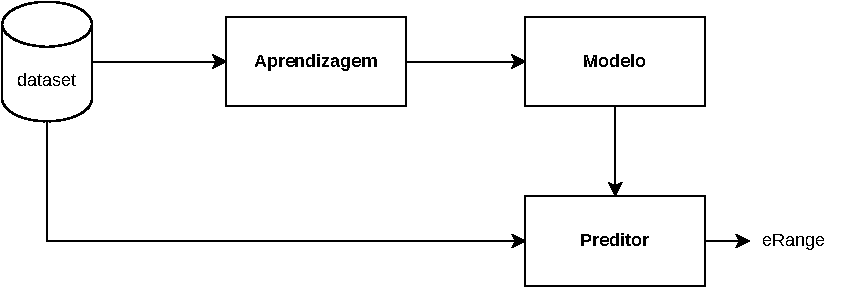
\includegraphics[width=0.90\textwidth]{./figures/objetivo_fase_de_geracao.pdf}
		
% 	};
% \end{tikzpicture}



%\vspace{1cm}
% \begin{itemize}
% 	\item Desenvolvimento de uma aplicação:
% 	\begin{itemize}
% 		\item Uso de aprendizagem automática (\textit{machine learning})
% 		para a resolução do problema
% 		\item Aprendizagem do modelo através de \textit{datasets}
% 		contendo os consumos em viagens efetuadas por carros eléctricos
% 	\end{itemize}
% \end{itemize}


\end{frame}

\subsection[Desafios de implementação]{Desafios de implementação}
\begin{frame}
\frametitle{Introdução - Desafios de implementação}

%\todo[inline]{TODO: imagem}

\begin{itemize}
	%\item Escassez de \textit{datasets} para testes de algoritmos - proteção proprietária
	\item Escassez de \textit{datasets} 
		  \begin{itemize}
				\item Protegidos - Competição comercial
			  	\item Necessários para teste de algoritmos
		  \end{itemize}
	\item Escolha dos algoritmos de \textit{machine learning}
	\item Dependência de vários fatores aumenta a complexidade do problema
	 \begin{itemize}
			\item Limitado aos fatores existentes nos \textit{datasets} - 
			\textit{SOC}, \textit{IEC}, etc
			\item Seleção de fatores mais relevantes% Reduzir complexidade de algoritmos
		  \end{itemize}
\end{itemize}

\end{frame}

\section[Estado da arte]{Estado da arte}
\subsection[\textit{Datasets}]{\textit{Datasets}}
\begin{frame}
\frametitle{Estado da arte - \textit{Datasets}}
\vspace{0.6cm}
\begin{itemize}
	\item \textit{EV Database} \footfullcite{onlineEvDatabase}
	- Características de carros elétricos
\end{itemize}
\vspace{0.5cm}
\begin{itemize}
	\item \textit{VED Dataset} \footfullcite{vedDatasetCleared}
		  - Dados de condução de um \textit{Nissan Leaf} (2013).
	\item \textit{Classic EV X Project} \footfullcite{classicEVXCleared}
	- Dados de condução de um BMW i3 94Ah (2016-2017) - obtidos por simulação.
	\item \textit{Emobpy} \footfullcite{emobpyCleared}
		  - Ferramenta de simulação de dados condução de veículos elétricos
\end{itemize}
\vspace{1cm}
\end{frame}

%\subsection[\textit{Datasets} de condução]{\textit{Datasets} de condução}
\begin{frame}
\frametitle{Estado da arte - \textit{Datasets}}

\begin{table}[]
	\centering
	\resizebox{\textwidth}{!}{%
	\begin{tabular}{|c|c|c|c|}
		\hline
							& VED dataset                                                                                                                                                                                        & Emobpy                                                                                                & \begin{tabular}[c]{@{}c@{}}Classic EV\\  X Project\end{tabular}                                           \\ \hline
		Tipo de viagens     & Reais                                                                                                                                                                                              & Simuladas                                                                                             & Simuladas                                                                                                 \\ \hline
		Número de viagens   & 507                                                                                                                                                                                                & Infinitas                                                                                             & 1                                                                                                         \\ \hline
		Modelos de veículos & 1                                                                                                                                                                                                  & 102                                                                                                   & 1                                                                                                         \\ \hline
		Parâmetros úteis    & \begin{tabular}[c]{@{}c@{}}velocidade, \\ estado de carga bateria,\\ potência do aquecimento,\\ potência do ar condicionado, \\ currente da bateria, \\ voltagem da bateria, \\ tempo\end{tabular} & \begin{tabular}[c]{@{}c@{}}distância, \\ consumo instantâneo,\\ potência média, \\ tempo\end{tabular} & \begin{tabular}[c]{@{}c@{}}consumo instantâneo,\\  bateria restante, \\ velocidade, \\ tempo\end{tabular} \\ \hline
	\end{tabular}
	}
	\end{table}
	

\end{frame}

\subsection[Implementacoes]{Implementações}
\begin{frame}[label={Implementacoes}]
\frametitle{Estado da arte - Implementações}

\let\oldfootnotesize\footnotesize
\renewcommand*{\footnotesize}{\oldfootnotesize\tiny}
\vspace{0.5cm}
\begin{itemize}
	\item Algoritmo básico
	\item Algoritmo baseado em historial com janela deslizante
	\item Uso combinado de \textit{Gradient Boosting Regression Trees}
		  \footfullcite{machineLearningERangeGradientBoostRtsCleared}
	\item \textit{Ensemble learning} \footfullcite{eRangeMachineLearningEnsembleCleared} com: 
		  \begin{itemize}
			  \item \textit{Decision Tree }
			  \item \textit{Random Forest}
			  \item \textit{K-Nearest Neighbor}
		  \end{itemize}
	\item \textit{Self-Organizing Maps}\footfullcite{eRangeMachineLearningGHSOMCleared} 
		  (e híbridos com \textit{Regression Trees} \footfullcite{machineLearningERangeSOMandRtsCleared})
	\item Redes neuronais com \textit{Multiple Linear Regression} 
		  \footfullcite{eRangeMachineLearningNeuralnetworkMLRCleared}
\end{itemize}
\vspace{0.5cm}

\renewcommand*{\footnotesize}{\oldfootnotesize}

\end{frame}

\section[Trabalho realizado]{Trabalho realizado}
\begin{frame}
\frametitle{Trabalho realizado}

\begin{itemize}
	\item Estudo do problema e soluções existentes
	\item Estudo de \textit{datasets}
	\item Implementação de dois algoritmos para cálculo do \textit{eRange}:
		  \begin{itemize}
		      \item Algoritmo "básico" 
			  \begin{itemize}
				  \item $eRange=\frac{FBE}{AEC} \cdot SOC [km]$
			  \end{itemize}
			  \item Algoritmo \textit{history-based} \footfullcite{classicEVXCleared2}
			  \begin{itemize}
				\item $eRange(k)=\frac{FBE}{\sum_{n=0}^{N-1} w_{i} \cdot  AEC(k-i)} \cdot SOC(k) [km]$
			\end{itemize}
		  \end{itemize}
\end{itemize}

\end{frame}

\begin{frame}
	\frametitle{Classic EV X Project \textit{Dataset} - BMW i3 94Ah}
	\framesubtitle{
		Algoritmo básico vs \textit{history-based} 
		\footfullcite{classicEVXCleared2}, \footfullcite{git}
	}
	\vspace{-0.5cm}
	\begin{figure}[H]
		\begin{center}
			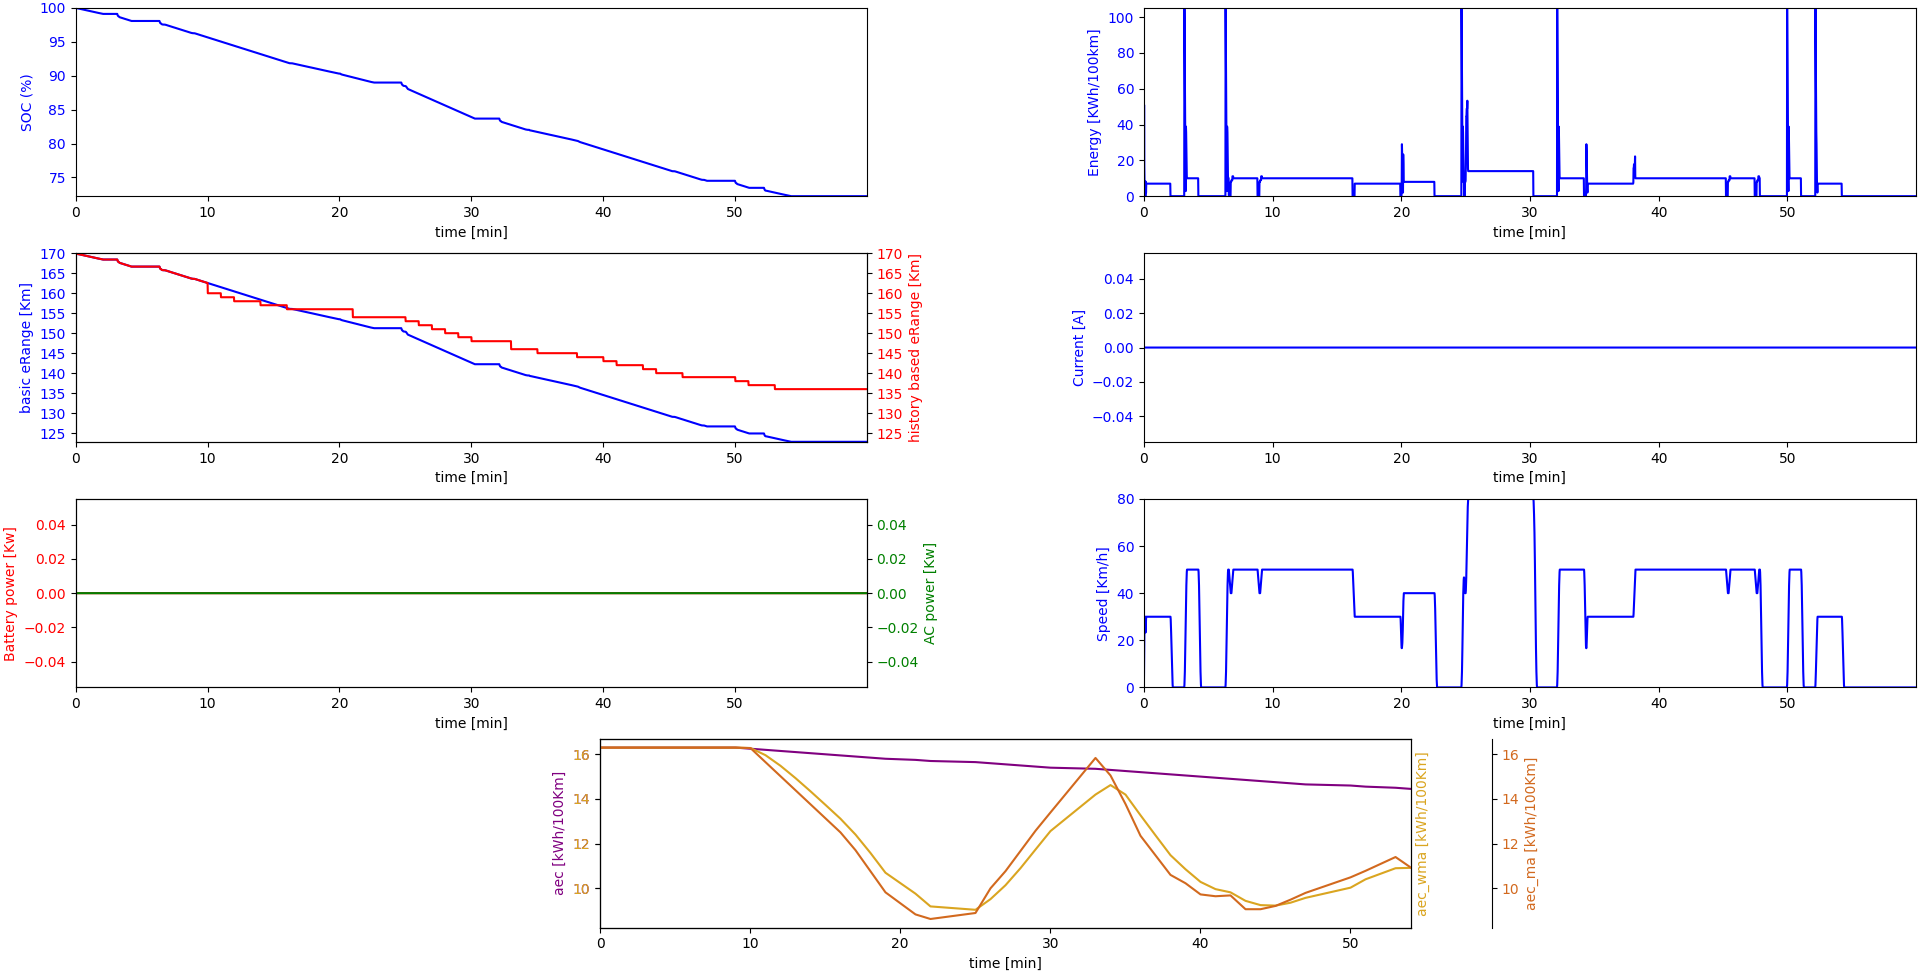
\includegraphics[scale=0.22]{./figures/demo_application_classic.png}
		\end{center}
	\end{figure}
	
\end{frame}

\begin{frame}
	\frametitle{VED \textit{Dataset} - \textit{Nissan Leaf}}
	\framesubtitle{
		Algoritmo básico vs \textit{history-based} 
		\footfullcite{classicEVXCleared2}, \footfullcite{git}
	}
	\vspace{-0.5cm}
	\begin{figure}[H]
		\begin{center}
			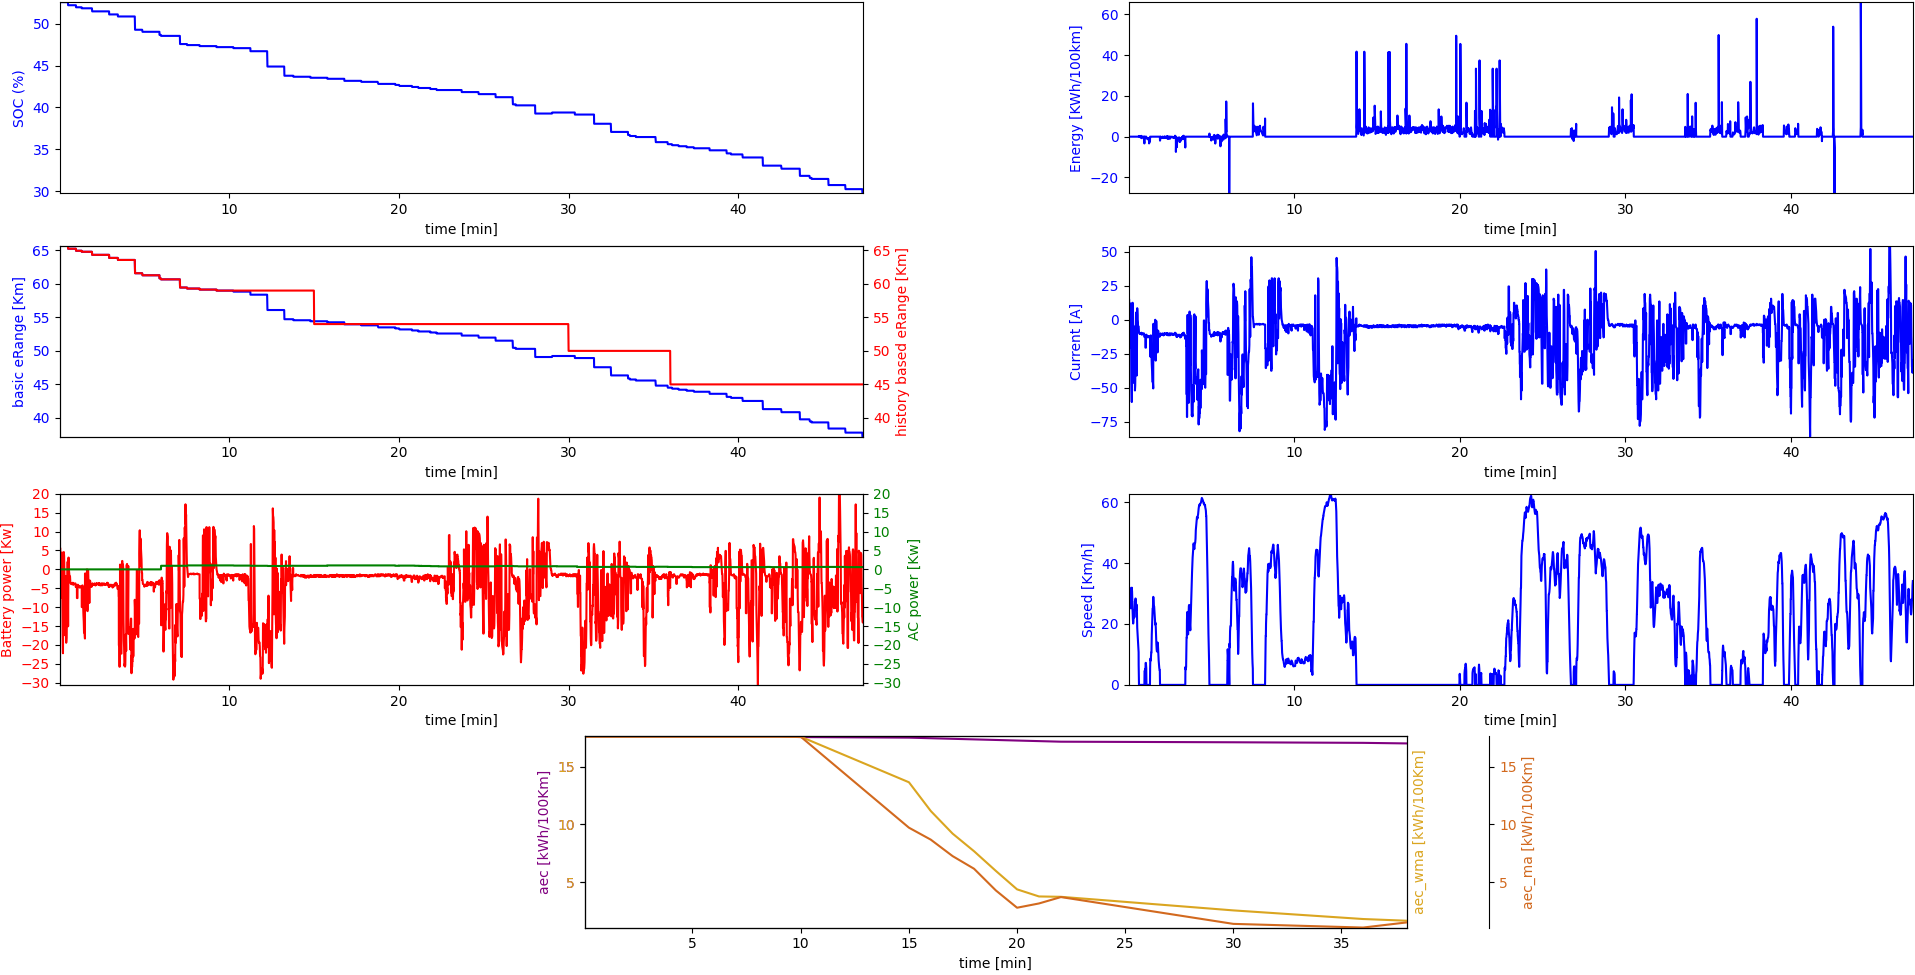
\includegraphics[scale=0.22]{./figures/demo_application_ved.png}
		\end{center}
	\end{figure}
	
\end{frame}

\section[Trabalho futuro]{Trabalho futuro}
\subsection{Objetivos}
\begin{frame}
\frametitle{Trabalho futuro}

\begin{itemize}
	\item Arquitetura de projeto
		  \begin{itemize}
			  \item Avaliação e escolha do algoritmo 
			  de \textit{machine learning}
		  \end{itemize} 
	\item Implementação da aplicação
		  \begin{itemize}
		      \item Integração do \textit{dataset}
		      \item Implementação do modelo
		      \item Comparação com modelos existentes
		  \end{itemize}
	\item Avaliação experimental
	\item Análise de resultados
	\item Conclusões
\end{itemize}

\end{frame}

\subsection{Diagrama de \textit{Gantt}}
\begin{frame}
\frametitle{Diagrama de \textit{Gantt}}

\begin{center}
	\begin{figure}[H]
		\begin{center}
			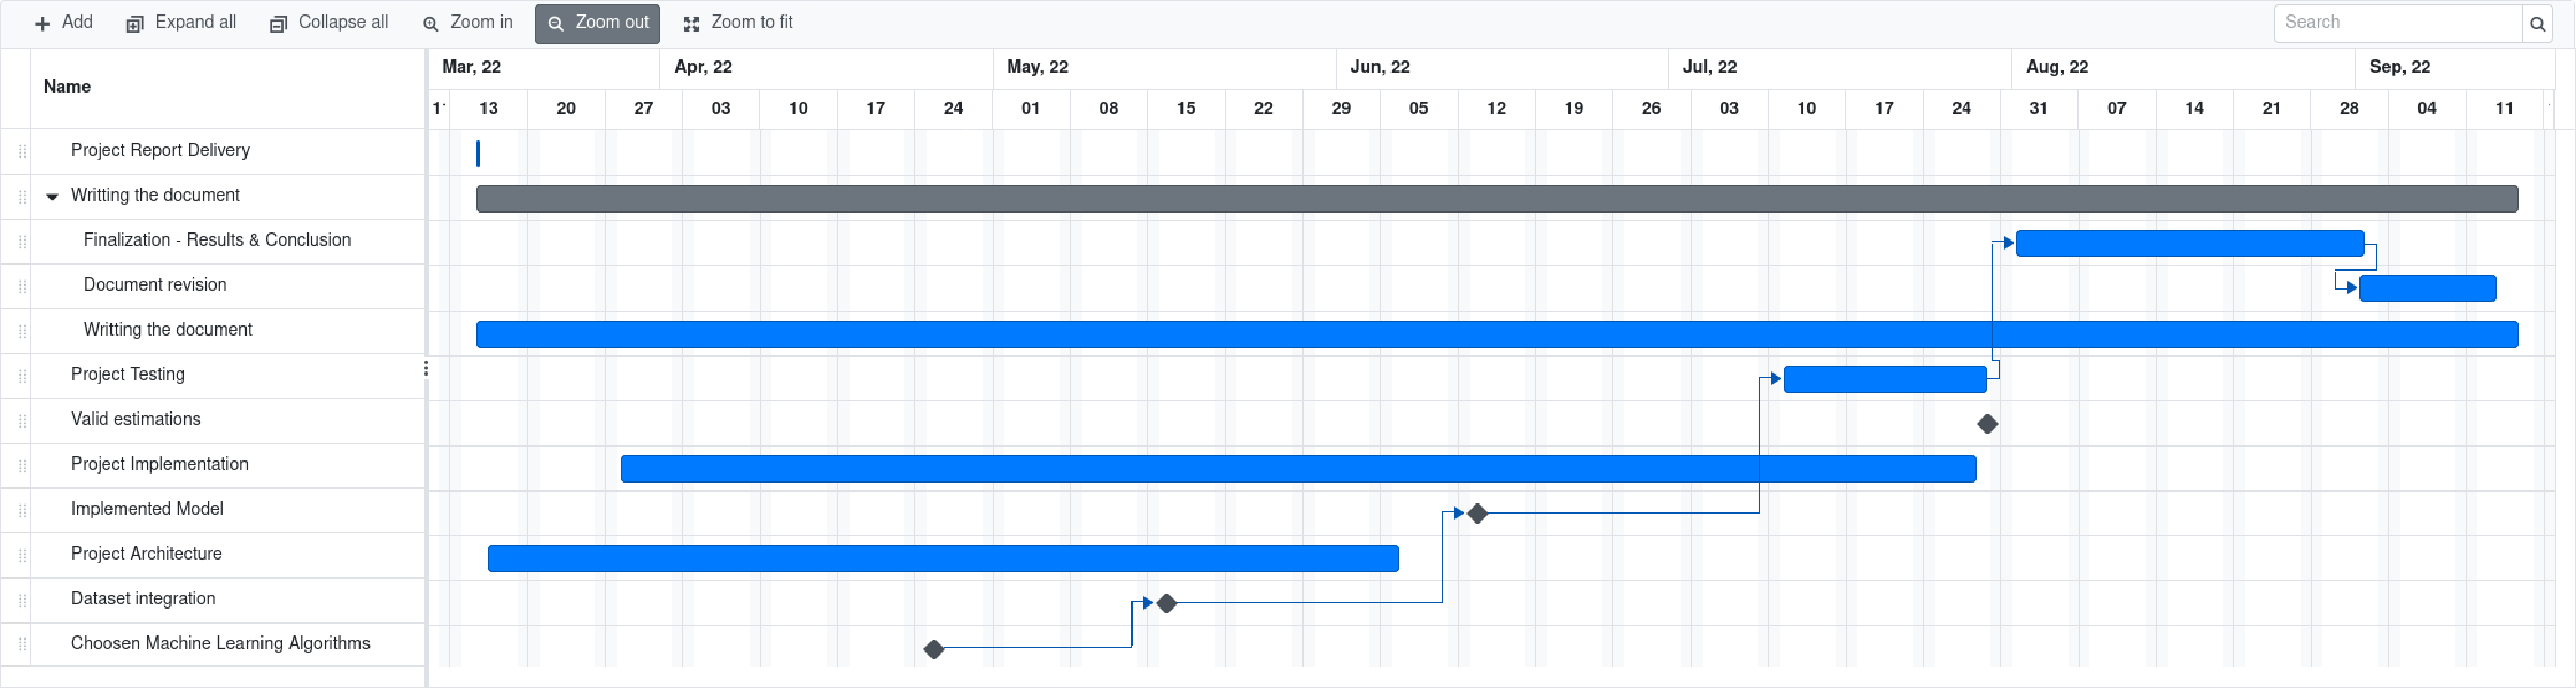
\includegraphics[scale=0.16]{./figures/planning_tiny1.pdf}
		\end{center}
	\end{figure}
\end{center}


\begin{figure}[H]
    \begin{center}
        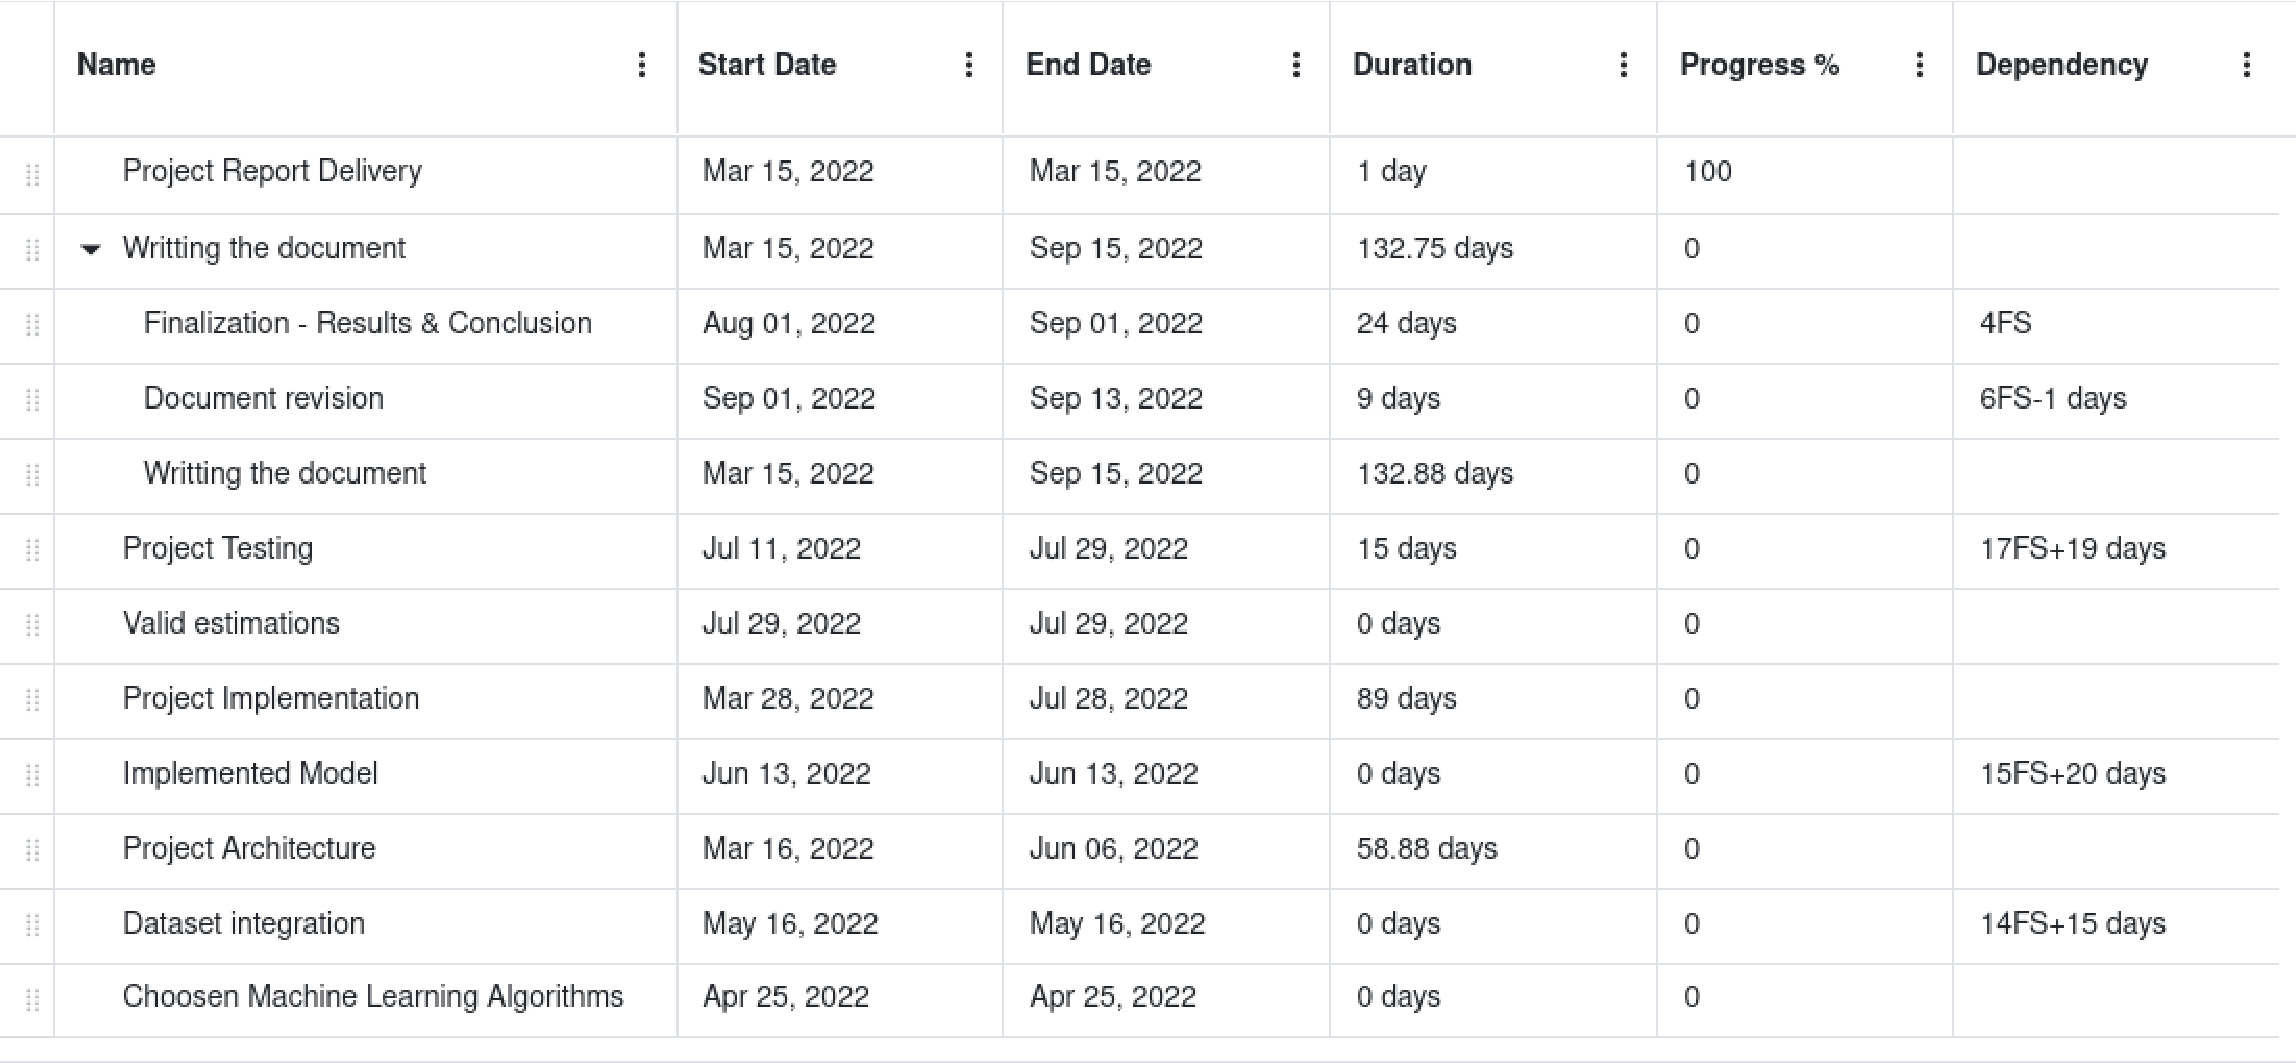
\includegraphics[scale=0.20]{./figures/planning_tiny2.pdf}
    \end{center}
\end{figure}

\end{frame}

\begin{frame}
	
	\vspace{1cm}
	\centering \resizebox{\linewidth}{2cm}{\itshape Obrigado}

\end{frame}

\begin{frame}
	\frametitle{System overview - Dataset generation}
	\vspace{0.5cm}
	\begin{figure}[H]
		\begin{center}
			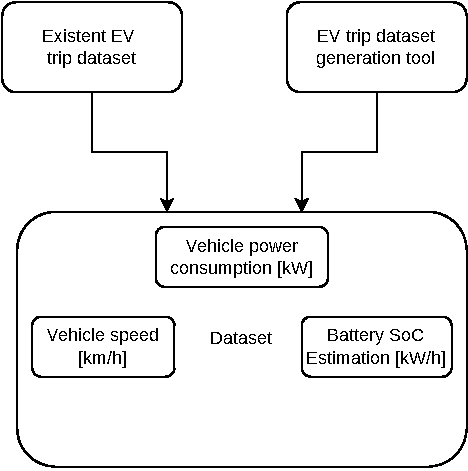
\includegraphics[scale=0.80]{./figures/report_generic_diagram_dataset_generation_phase.pdf}
		\end{center}
	\end{figure}
	
\end{frame}

\begin{frame}
	\frametitle{System overview - Learning phase}
	\vspace{0.5cm}
	\begin{figure}[H]
		\begin{center}
			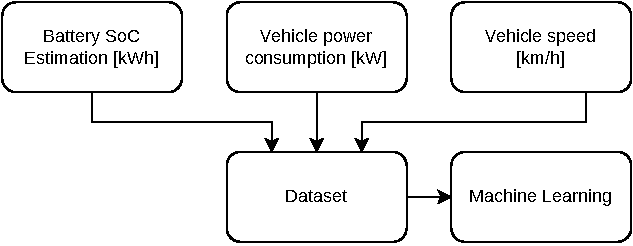
\includegraphics[scale=0.80]{./figures/report_generic_diagram_learn_phase.pdf}
		\end{center}
	\end{figure}
	
\end{frame}

\begin{frame}
	\frametitle{System overview - Estimation phase}
	\vspace{0.5cm}
	\begin{figure}[H]
		\begin{center}
			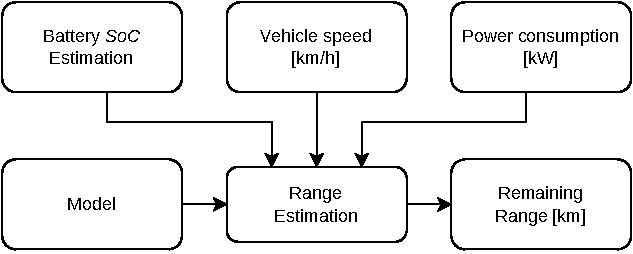
\includegraphics[scale=0.80]{./figures/report_generic_diagram_estimation_phase.pdf}
		\end{center}
	\end{figure}
	
\end{frame}

\end{document}